\documentclass[12pt]{article}
\usepackage[usenames]{color} %used for font color
\usepackage{amsmath,amssymb,amsthm,amsfonts} %maths
\usepackage[utf8]{inputenc} %useful to type directly accentuated characters
\usepackage{hyperref}
\usepackage[top=1in, bottom = 1in, left = 0.75in, right = 0.75in]{geometry}
\usepackage{graphicx,subcaption}
\usepackage{tcolorbox}
\usepackage{listings}
\usepackage{booktabs, multirow, multicol}

\definecolor{codegreen}{rgb}{0,0.6,0}
\definecolor{codegray}{rgb}{0.5,0.5,0.5}
\definecolor{codepurple}{rgb}{0.58,0,0.82}
\definecolor{backcolour}{rgb}{0.95,0.95,0.92}

\lstdefinestyle{mystyle}{
    backgroundcolor=\color{backcolour},   
    commentstyle=\color{codegreen},
    keywordstyle=\color{magenta},
    numberstyle=\tiny\color{codegray},
    stringstyle=\color{codepurple},
    basicstyle=\ttfamily\footnotesize,
    breakatwhitespace=false,         
    breaklines=true,                 
    captionpos=b,                    
    keepspaces=true,                 
    numbers=left,                    
    numbersep=5pt,                  
    showspaces=false,                
    showstringspaces=false,
    showtabs=false,                  
    tabsize=2
}

\lstset{style=mystyle}

\setlength\parindent{0pt}


\newtheoremstyle{problemstyle}  							% <name>
        {3pt}                                               % <space above>
        {3pt}                                               % <space below>
        {\normalfont}                               		% <body font>
        {}                                                  % <indent amount}
        {\bfseries}                 						% <theorem head font>
        {\normalfont\bfseries.}         					% <punctuation after theorem head>
        {.5em}                                          	% <space after theorem head>
        {}                                                  % <theorem head spec (can be left empty, meaning `normal')>
\theoremstyle{problemstyle}

\newtheorem{pbm}{Problem}
\newtheorem{solution}{Solution}
\newtheorem*{solution*}{Solution}

\newenvironment{problem}{
\begin{tcolorbox}[colback=green!10!white,colframe=black!75!black, parbox = false]\begin{pbm} }{\end{pbm}\end{tcolorbox} }


\makeatletter
\newcommand*\bigcdot{\mathpalette\bigcdot@{.5}}
\newcommand*\bigcdot@[2]{\mathbin{\vcenter{\hbox{\scalebox{#2}{$\m@th#1\bullet$}}}}}
\makeatother


\newcommand{\prob}{\mathbb{P}}
\newcommand{\E}{\mathbb{E}}
\newcommand{\Var}{\mathbb{V}}
\newcommand{\normal}{\mathcal{N}}
\newcommand{\Sample}{\mathcal{S}}
\newcommand{\R}{\mathbb{R}}
\newcommand{\C}{\mathbb{C}}
\newcommand{\N}{\mathbb{N}}
\newcommand{\Q}{\mathbb{Q}}
\newcommand{\Z}{\mathbb{Z}}
\newcommand{\indep}{\mathrel{\text{\scalebox{1.07}{$\perp\mkern-10mu\perp$}}}}
\newcommand{\ind}[1]{\mathbf{1}_{ \{#1\} }}


\begin{document}

\begin{titlepage}
    \begin{center}
        \vspace*{3cm}
        \Huge{\textbf{Survival Analysis Assignment 1}}\\
        \vspace*{1cm}
        \large{\textit{Master of Statistics (M.Stat.) Year II, Session 2020-21}}\\
        \vspace*{5cm}
        \begin{tcolorbox}[colback=black!5!white,colframe=black!75!black, width = 0.5\linewidth]
            \vspace*{0.5cm}
            \textbf{Name: } Subhrajyoty Roy\\
            \textbf{Roll: } MB1911
            \vspace*{0.5cm}
        \end{tcolorbox}
    \end{center}
    \vspace*{3cm}
    \begin{flushright}
        \large\textit{\today}
    \end{flushright}
\end{titlepage}

\begin{problem}
    Compare performances of the exact confidence interval for the parameter $\theta$ for Type 2 censoring scheme and different asymptotic confidence intervals for $\theta$ for Type 1 censoring scheme when the lifetime distribution is an exponential distribution with mean $\theta$. 
\end{problem}

\begin{solution*}
    Let, $r$ denotes the total number of failures and $V$ denotes the total time on tests. Under both censoring scheme, the maximum likelihood estimate of $\theta$ is given by $\widehat{\theta} = V/r$. 

    In Type 2 censoring case, the exact $100(1-\alpha)\%$ confidence interval for $\theta$ is given by 

    $$
    CI_5 = \left( \dfrac{2r\widehat{\theta}}{\chi^2_{2r, 1-\alpha/2}}, \dfrac{2r\widehat{\theta}}{\chi^2_{2r, \alpha/2}} \right),
    $$

    \noindent where $\chi^2_{a, \alpha}$ denotes the $\alpha$-th quantile of chi-squared distribution with $a$ degrees of freedom. 

    On the other hand, for Type 1 censoring scheme, $4$ types of asymptotic $100(1-\alpha)\%$ confidence interval exist.

    \begin{enumerate}
        \item Based on the expected Fisher's information, one has 
        $$
        CI_1 = \left( \widehat{\theta} - \dfrac{z_{1 - \alpha/2}}{\sqrt{n}} \dfrac{\widehat{\theta}}{\sqrt{1 - \exp\left[ -T_0/\widehat{\theta} \right]}}, \widehat{\theta} + \dfrac{z_{1 - \alpha/2}}{\sqrt{n}} \dfrac{\widehat{\theta}}{\sqrt{1 - \exp\left[ -T_0/\widehat{\theta} \right]}} \right),
        $$
        \noindent where $z_{1 - \alpha/2}$ is the $(1 - \alpha/2)$-th quantile of the standard normal distribution.
        \item Similar confidence interval based on the observed Fisher's information is given by 
        $$
        CI_2 = \left( \widehat{\theta} - \dfrac{z_{1 - \alpha/2}}{\sqrt{r}} \widehat{\theta} , \widehat{\theta} + \dfrac{z_{1 - \alpha/2}}{\sqrt{r}} \widehat{\theta} \right).
        $$
        \item Cox (1953) proposed another confidence interval as 
        $$
        CI_3 = \left( \dfrac{2r\widehat{\theta}}{\chi^2_{2r+1, 1-\alpha/2}}, \dfrac{2r\widehat{\theta}}{\chi^2_{2r+1, \alpha/2}} \right)
        $$
        \item Based on likelihood ratio test for $H_0: \theta = \theta_0$, one may obtain that 
        $$
        \prob\left( 2r \log({\theta}) + 2\dfrac{\sum_{i=1}^n x_i}{{\theta}} < \chi^2_{1, 1-\alpha} + 2r\log(\widehat{\theta}) + 2r \right) \approx (1 - \alpha),
        $$
        \noindent where $x_i$ is the $i$-th censored lifetime. Hence, one can numerically invert this to obtain bounds for $\theta$ such that $\prob(L(\widehat{\theta})< \theta < U(\widehat{\theta})) \approx (1 - \alpha)$, which gives an approximate confidence interval as $CI_4 = (L(\widehat{\theta}), U(\widehat{\theta}))$.
    \end{enumerate}

To compare performances between these two different setups, we choose $r$ in Type 2 censoring as $\left[ n(1 - \exp(-T_0/\theta)) \right]$ which is the expected number of failures under Type 1 censoring. To compare between different confidence interval schemes, we obtain $B = 1000$ resamples of sample size $n$ (to be varied) and compute the confidence intervals based on each of these schemes, and finally obtain the approximate coverage probability (proportion of $B$ resamples for which the confidence interval contains the true value of $\theta$) and average length of the intervals (averaged over all $B$ resamples). We shall choose $T_0$ to be such that a pre-defined proportion of samples in expectation is censored, $e^{-T_0/\theta} = p$, i.e. $T_0 = \theta \log(1/p)$, where $p$ is a pre-defined constant ($5\%, 10\%$ and $20\%$). As true parameter $\theta$, we choose $\theta = 1$ and to see the effect of the sample size, we choose $n = 5, 10, 25, 50, 100$. Table~\ref{tbl:ci-1} and Table~\ref{tbl:ci-2} contains the detailed description of the approximate coverage probabilities and the average length of the confidence intervals under different censoring proportion $p$ and sample size $n$.


\begin{table}[ht]
    \centering
    \begin{tabular}{llrrrrr}
        \toprule
        Proportion of Censoring ($\mathbf{p}$) & Sample size ($\mathbf{n}$) & $\mathbf{CI_1}$ & $\mathbf{CI_2}$ & $\mathbf{CI_3}$ & $\mathbf{CI_4}$ & $\mathbf{CI_5}$\\
        \midrule
        \multirow{5}{*}{$5\%$} & 5 & 0.848 & 0.847 & 0.936 & 0.943 & 0.949 \\
        & 10 & 0.894 & 0.894 & 0.936 & 0.942 & 0.939 \\
        & 25 & 0.938 & 0.94 & 0.945 & 0.949 & 0.955 \\
        & 50 & 0.951 & 0.953 & 0.956 & 0.959 & 0.954 \\
        & 100 & 0.949 & 0.949 & 0.953 & 0.952 & 0.952 \\
        \midrule
        \multirow{5}{*}{$10\%$} & 5 & 0.849 & 0.847 & 0.936 & 0.942 & 0.952 \\
        & 10 & 0.891 & 0.894 & 0.939 & 0.945 & 0.95 \\
        & 25 & 0.936 & 0.935 & 0.949 & 0.95 & 0.956 \\
        & 50 & 0.949 & 0.948 & 0.961 & 0.959 & 0.955 \\
        & 100 & 0.95 & 0.949 & 0.954 & 0.955 & 0.951 \\
        \midrule
        \multirow{5}{*}{$20\%$} & 5 & 0.856 & 0.85 & 0.938 & 0.941 & 0.952 \\
        & 10 & 0.897 & 0.9 & 0.943 & 0.946 & 0.952 \\
        & 25 & 0.939 & 0.94 & 0.957 & 0.959 & 0.961 \\
        & 50 & 0.947 & 0.95 & 0.966 & 0.967 & 0.954 \\
        & 100 & 0.947 & 0.947 & 0.945 & 0.944 & 0.943 \\
        \bottomrule
    \end{tabular}
    \caption{Approximate coverage probabilities of different confidence intervals}
    \label{tbl:ci-1}
\end{table}

\begin{table}[ht]
    \centering
    \begin{tabular}{llrrrrr}
        \toprule
        Proportion of Censoring ($\mathbf{p}$) & Sample size ($\mathbf{n}$) & $\mathbf{CI_1}$ & $\mathbf{CI_2}$ & $\mathbf{CI_3}$ & $\mathbf{CI_4}$ & $\mathbf{CI_5}$\\
        \midrule
        \multirow{5}{*}{$5\%$} & 5 & 1.839 & 1.828 & 2.31 & 2.403 & 3.857 \\
        & 10 & 1.282 & 1.279 & 1.438 & 1.489 & 1.756 \\
        & 25 & 0.808 & 0.807 & 0.846 & 0.856 & 0.918 \\
        & 50 & 0.572 & 0.571 & 0.585 & 0.589 & 0.608 \\
        & 100 & 0.404 & 0.403 & 0.408 & 0.409 & 0.417 \\
        \midrule
        \multirow{5}{*}{$10\%$} & 5 & 1.984 & 1.976 & 2.57 & 2.32 & 5.568 \\
        & 10 & 1.338 & 1.336 & 1.515 & 1.573 & 1.928 \\
        & 25 & 0.836 & 0.835 & 0.878 & 0.89 & 0.973 \\
        & 50 & 0.59 & 0.589 & 0.604 & 0.608 & 0.631 \\
        & 100 & 0.416 & 0.415 & 0.42 & 0.422 & 0.43 \\
        \midrule
        \multirow{5}{*}{$20\%$} & 5 & 2.255 & 2.241 & 3.112 & 1.955 & 5.568 \\
        & 10 & 1.452 & 1.446 & 1.672 & 1.749 & 2.166 \\
        & 25 & 0.896 & 0.895 & 0.947 & 0.962 & 1.038 \\
        & 50 & 0.629 & 0.629 & 0.647 & 0.651 & 0.675 \\
        & 100 & 0.443 & 0.443 & 0.449 & 0.451 & 0.458 \\
        \bottomrule
    \end{tabular}
    \caption{Average length of the different confidence intervals}
    \label{tbl:ci-2}
\end{table}

From the metrics shown in Table~\ref{tbl:ci-1} and Table~\ref{tbl:ci-2}, we may conclude the following.

\begin{enumerate}
    \item As the sample size $n$ increases, all of these confidence intervals perform equivalently, since all of these confidence intervals are asymptotically equivalent.
    \item For small sample sizes, Cox's confidence interval and the interval obtained through LRT approximately attains the $95\%$ coverage probability. The exact confidence interval for Type 2 censoring almost always attains the $95\%$ coverage probability irrespective of the sample size and proportion of censoring.
    \item Proportion of censoring do not have a considerable effect on the coverage probabilities. However, the length of the confidence intervals increases as proportion of censored datapoint increases.
    \item In terms of length of the confidence intervals, the exact confidence interval for Type 2 censoring ($\text{CI}_5$) has highest length. Asymptotic CI's based on observed and expected information matrix have similar lengths.
    \item As the sample size increases, the length of the confidence interval shrinks for each of the method. 
\end{enumerate}

In summary, for small samples, $\text{CI}_1$ and $\text{CI}_2$ based on observed and expected Fisher's information matrix performs poorly, whereas, Cox's confidence interval and the CI obtained from inverting LRT performs better. The exact CI based on Type 2 censoring achieves the correct coverage probability, but at the cost of a longer interval.

\end{solution*}


\pagebreak

\begin{problem}
    Compare finite sample performances of the different asymptotic tests for $H_0 : \lambda = 1$ vs $H_1 : \lambda \neq 1$ under random censoring scheme where the lifetime distribution is $\exp(\lambda)$ ($\lambda$ is the rate parameter).
\end{problem}

\begin{solution*}
    Let $d$ denotes the total number of failures and $V$ denotes the total time on tests. Then, under random censoring scheme where the lifetime distribution is exponential with rate parameter $\lambda$, the maximum likelihood estimator of $\lambda$ is $\widehat{\lambda} = d/V$. Based on this, there are three types of asymptotic tests for testing the null hypothesis $H_0 : \lambda = \lambda_0$ vs $H_1 : \lambda \neq \lambda_0$. 

    \begin{enumerate}
        \item \textbf{Score Test} at level-$\alpha$ rejects the null hypothesis if 
        $$
        T_s = \dfrac{(d - V\lambda_0)^2}{d} \dfrac{\widehat{\lambda}^2}{\lambda_0^2} > \chi^2_{1, 1-\alpha}
        $$
        \noindent where $\chi^2_{1, 1-\alpha}$ is the $(1 - \alpha)$-th quantile of $\chi^2$ distribution with $1$ degrees of freedom.
        \item \textbf{Wald's Test} at level-$\alpha$ rejects the null hypothesis if 
        $$
        T_w = \dfrac{(d - V\lambda_0)^2}{d} > \chi^2_{1, 1-\alpha}
        $$
        \item \textbf{Likelihood Ratio Test (LRT)} at level-$\alpha$ rejects the null hypothesis if 
        $$
        T_{LR} = 2(\lambda_0 - \widehat{\lambda})V - 2d\log\left( \dfrac{\lambda_0}{\widehat{\lambda}} \right) > \chi^2_{1, 1-\alpha}
        $$
    \end{enumerate}

    To compare performances of these tests, without loss of generality we fix $\alpha = 0.05$ and $\lambda_0 = 1$. Then, we perform $B$ resamples, where in each of the resamples, we generate data according to the random censoring scheme for a range of values of $\lambda$, and then note where the aforementioned tests rejects or fails to reject the null hypothesis. Then, we can approximate the power of a test at $\lambda = \lambda_i$ as the proportion of resamples where the test rejects the null hypothesis for datasets generated from $\lambda = \lambda_i$. While this gives us an approximate power curve for each of these tests, we consider two metrices for ease of comparison.

    \begin{enumerate}
        \item The approximate size of the test i.e. the proportion of resamples for which a test rejects the null hypothesis when the data is generated from the parameter setting $\lambda = 1$.
        \item The approximate area under the power curve, for which we shall use trapezoidal rule, i.e. 
        $$
        \int_1^{\lambda_{\max}} \text{Power}(\lambda) d\lambda \approx \dfrac{1}{2(\Delta \lambda)} \left( \text{Power}(\lambda_1) + 2 \text{Power}(\lambda_2) + \dots + 2\text{Power}(\lambda_{n-1}) + \text{Power}(\lambda_n) \right)
        $$
        \noindent Since this area depends on the choice of $\lambda_{\max}$, the maximum value of $\lambda$ under the alternative, we consider $\dfrac{1}{\lambda_{\max}}\int_1^{\lambda_{\max}} \text{Power}(\lambda) d\lambda$ instead which will reside between $0$ and $1$.
    \end{enumerate}

    Now, finally for sample sizes, we shall use $n = 5, 10$ and $25$. Let $T$ and $C$ denote the random variables denoting lifetime and censoring. Then, we consider three different types of distribution for censoring.

    \begin{enumerate}
        \item If $C \sim \exp(\tau)$ be the censoring distribution, then the expected proportion of censoring is 
        $$
        \prob(T > C) = \int_0^\infty e^{-\lambda c}\tau e^{-\tau c} dc = \dfrac{\tau}{\tau + \lambda}
        $$
        \noindent Therefore, once we fix $p$ as the expected proportion of censoring, then we choose $\tau = p\lambda/(1- p)$.
        \item If $C \sim \text{Unif}(0, \theta)$, then 
        $$
        \prob(T > C) = \int_0^\theta e^{-\lambda c}\theta^{-1} dc = \dfrac{(1 - e^{-\lambda \theta})}{\theta} \approx \dfrac{\lambda \theta - \lambda^2\theta^2/2}{\theta} = \lambda - \dfrac{\lambda^2}{2}\theta
        $$
        \noindent Therefore, fixing the expected proportion of censoring as $p$, we may choose $\theta = 2(\lambda - p)/\lambda^2$.
        \item If $C \sim \text{Weibull}(\tau, 2)$, then 
        $$
        \prob(T > C) = 1 - \prob(T \leq C) = 1 - \int_0^\infty \lambda e^{-(\tau t)^2 - \lambda t} dt = 1 - \dfrac{\sqrt{\pi}}{\tau}e^{\lambda^2/2\tau^2} \left( 1 - \Phi(\lambda/2\tau) \right) 
        $$
        \noindent where $\Phi$ is the normal cdf. We can fix this probability as $p$ and numerically solve for $\tau$ to obtain the required parameter of Weibull distribution.
    \end{enumerate}

    We shall consider only 3 proportion of censoring, namely $5\%, 20\%$ and $40\%$. The performances of these tests when the censoring distribution is exponential, are tabulated in Table~\ref{tbl:test-exp}. Figure~\ref{fig:1} shows the approximate power curve of the aforementioned asymptotic tests under different sample sizes, where the censoring distribution is exponential with the parameter adjusted so that the expected censoring proportion is $5\%$. 

    \begin{table}[ht]
        \centering
        \begin{tabular}{@{}cl|rrr|rrr@{}}
            \toprule
            \multirow{2}{*}{\begin{tabular}[c]{@{}c@{}}Proportion of\\ Censoring\end{tabular}} & \multicolumn{1}{c|}{\multirow{2}{*}{n}} & \multicolumn{3}{c|}{Approximate Size} & \multicolumn{3}{c}{Area under the power curve} \\
             & \multicolumn{1}{c|}{} & \multicolumn{1}{c}{Score test} & \multicolumn{1}{c}{Wald's test} & \multicolumn{1}{c|}{LRT} & \multicolumn{1}{c}{Score test} & \multicolumn{1}{c}{Wald's test} & \multicolumn{1}{c}{LRT} \\ \midrule
            \multirow{3}{*}{$5\%$} & 5 & 0.153 & 0.027 & 0.057 & 0.846 & 0.394 & 0.798 \\
             & 10 & 0.106 & 0.035 & 0.057 & 0.859 & 0.811 & 0.846 \\
             & 25 & 0.074 & 0.04 & 0.048 & 0.866 & 0.861 & 0.864 \\ 
            \midrule
            \multirow{3}{*}{$20\%$} & 5 & 0.158 & 0.04 & 0.053 & 0.832 & 0.2 & 0.748 \\
            & 10 & 0.115 & 0.047 & 0.051 & 0.852 & 0.748 & 0.831 \\
            & 25 & 0.073 & 0.045 & 0.047 & 0.865 & 0.856 & 0.862 \\ 
            \midrule
            \multirow{3}{*}{$40\%$} & 5 & 0.148 & 0.047 & 0.056 & 0.802 & 0.064 & 0.647 \\
            & 10 & 0.116 & 0.053 & 0.041 & 0.84 & 0.56 & 0.79 \\
            & 25 & 0.076 & 0.049 & 0.043 & 0.861 & 0.839 & 0.854 \\
            \bottomrule
        \end{tabular}
        \caption{Small sample performances of score test, Wald's test and LRT for exponential distribution as the censoring distribution.}
        \label{tbl:test-exp}
    \end{table}

    \begin{figure}
        \centering
        \begin{subfigure}{0.75\textwidth}
            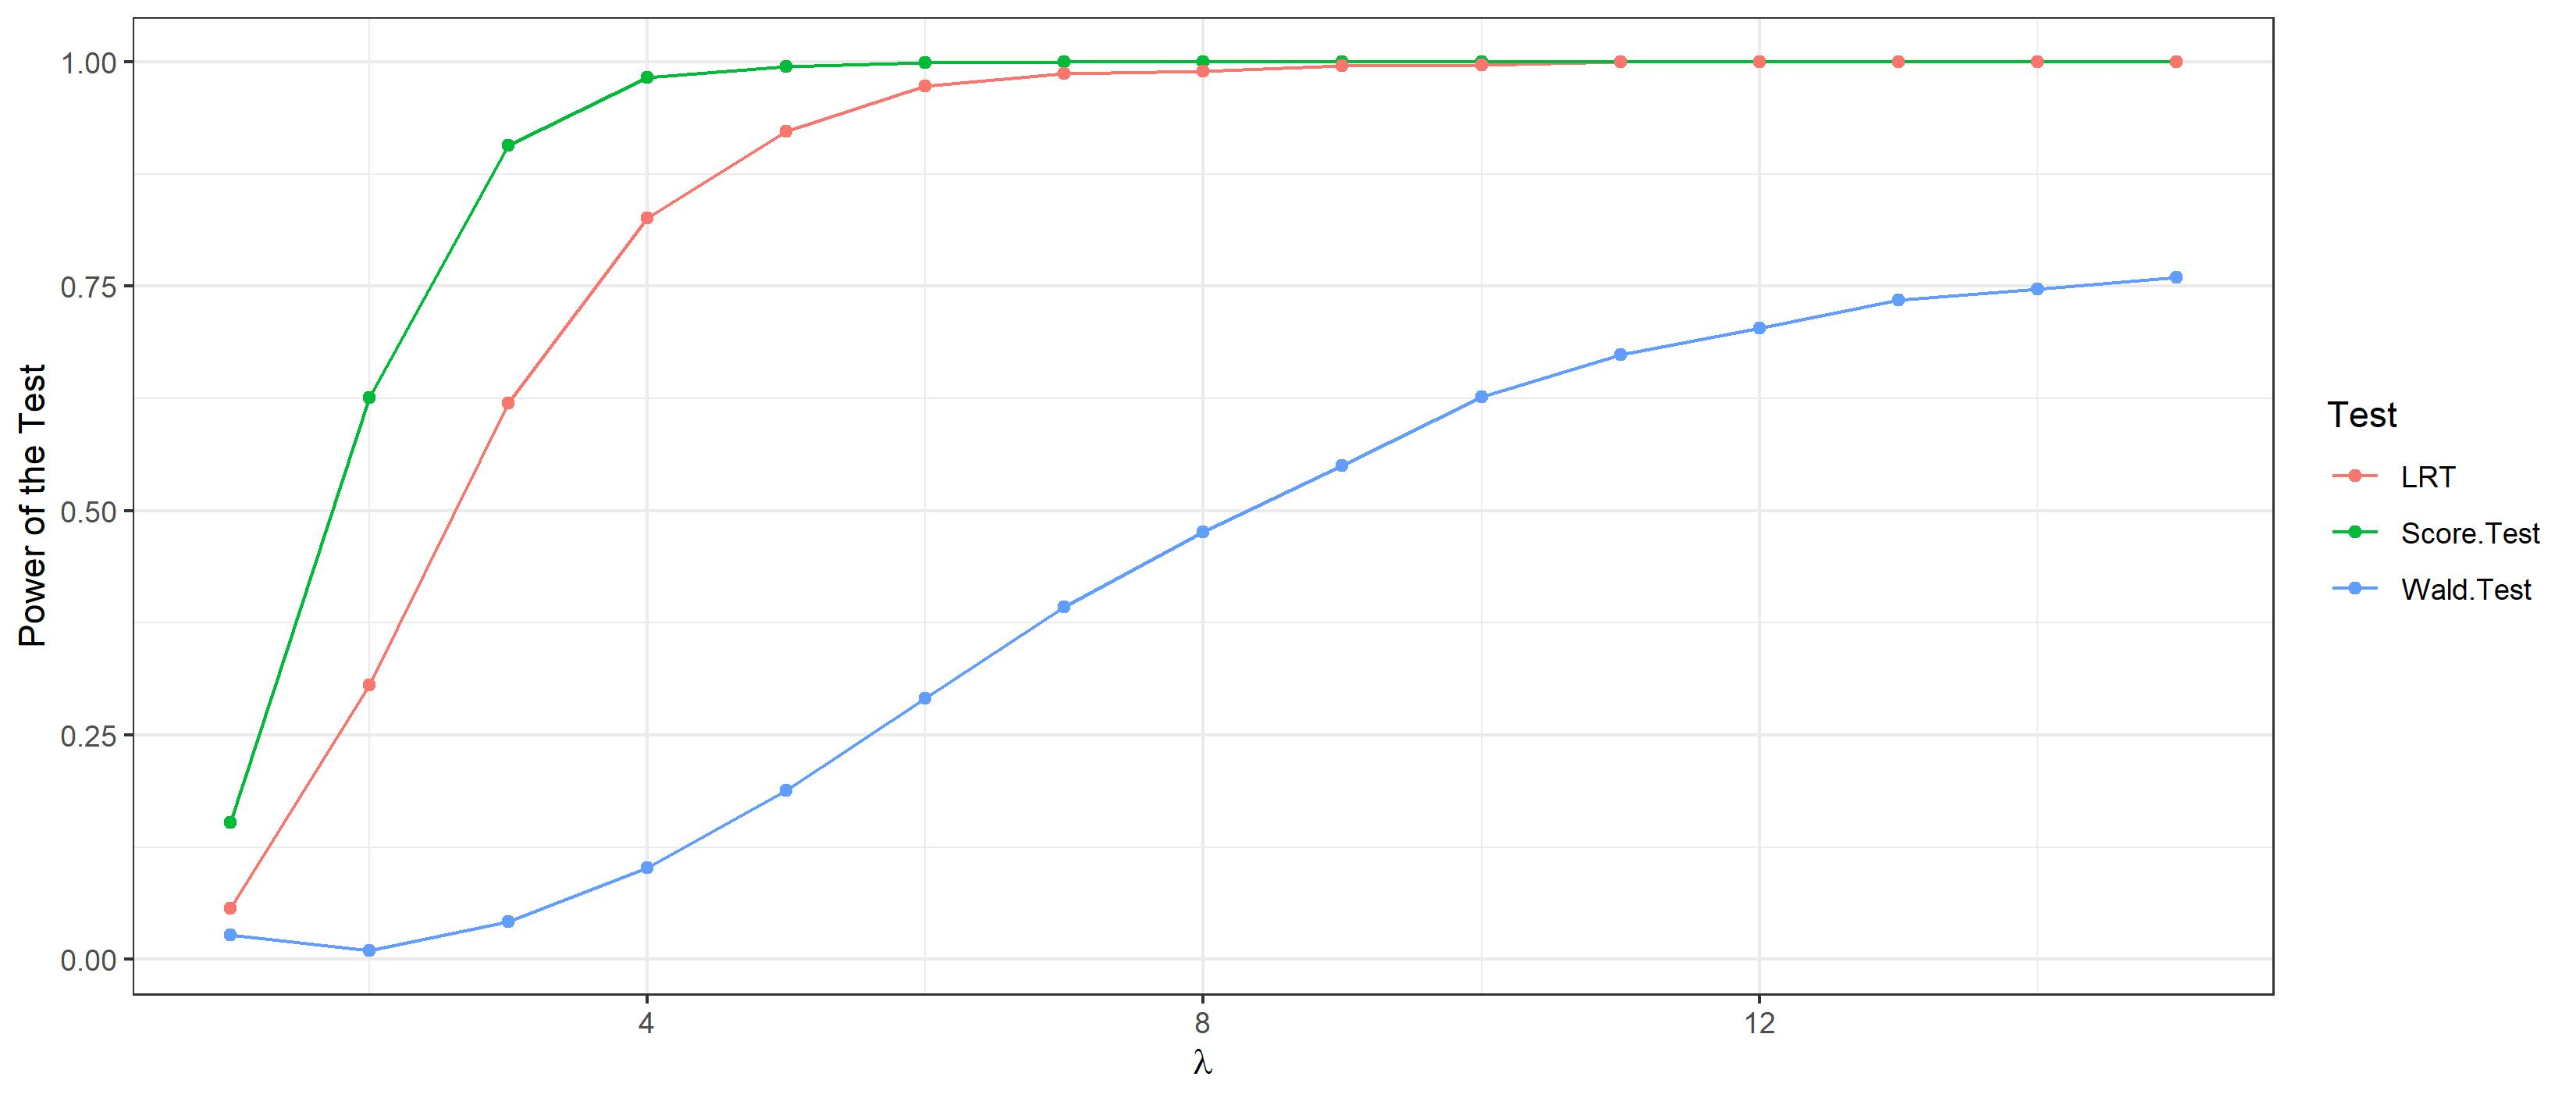
\includegraphics[width = \textwidth]{ExpTest-0.05-5.jpg}
            \caption{n = 5}
        \end{subfigure}
        \begin{subfigure}{0.75\textwidth}
            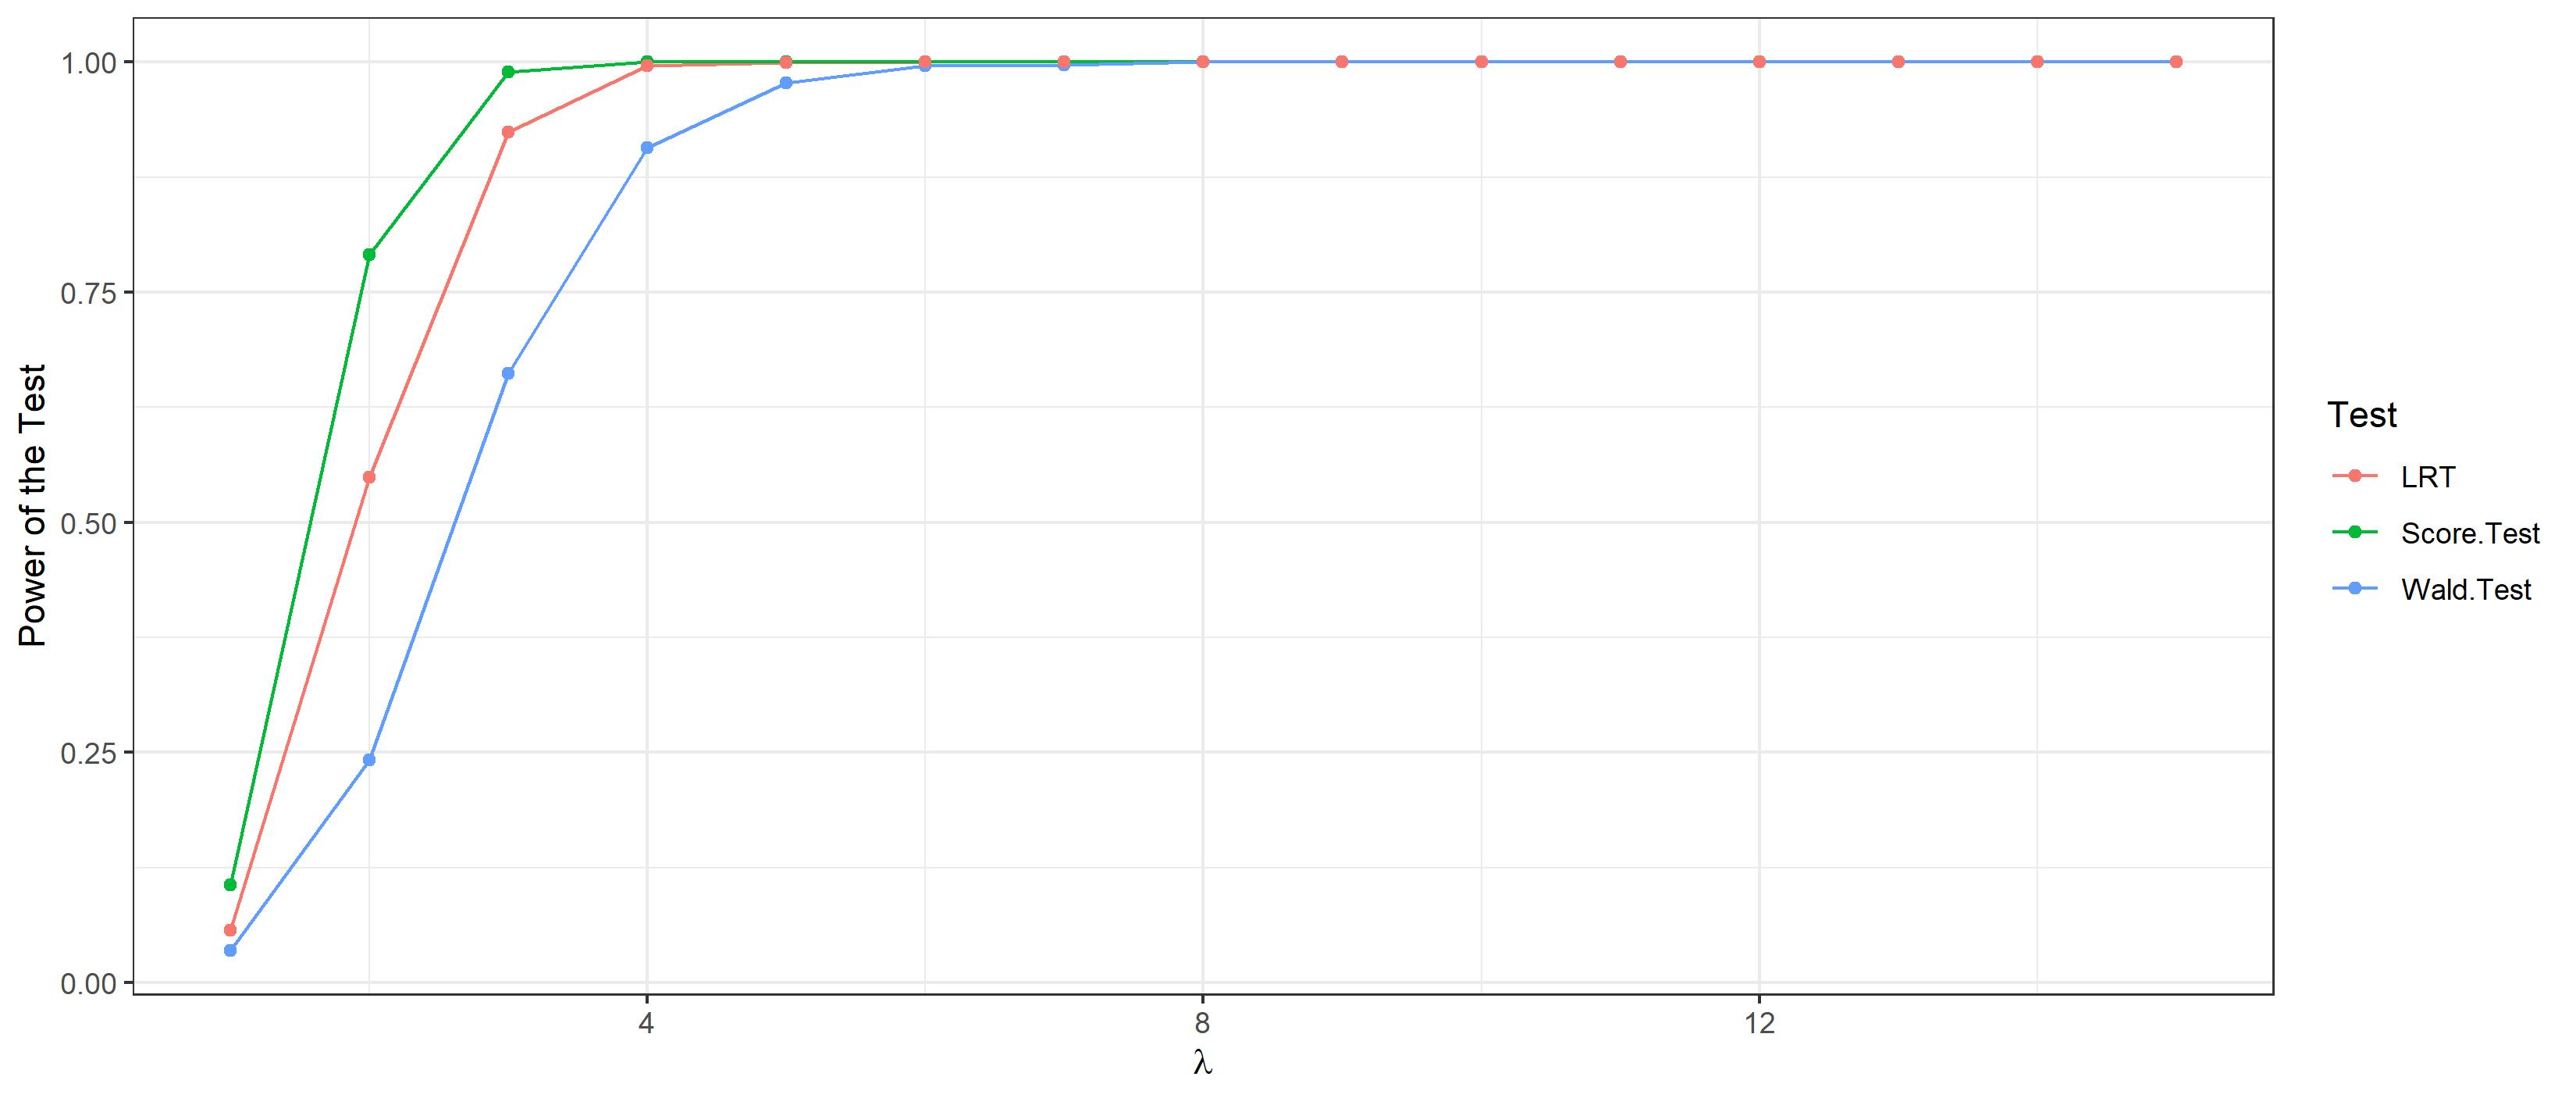
\includegraphics[width = \textwidth]{ExpTest-0.05-10.jpg}
            \caption{n = 10}
        \end{subfigure}
        \begin{subfigure}{0.75\textwidth}
            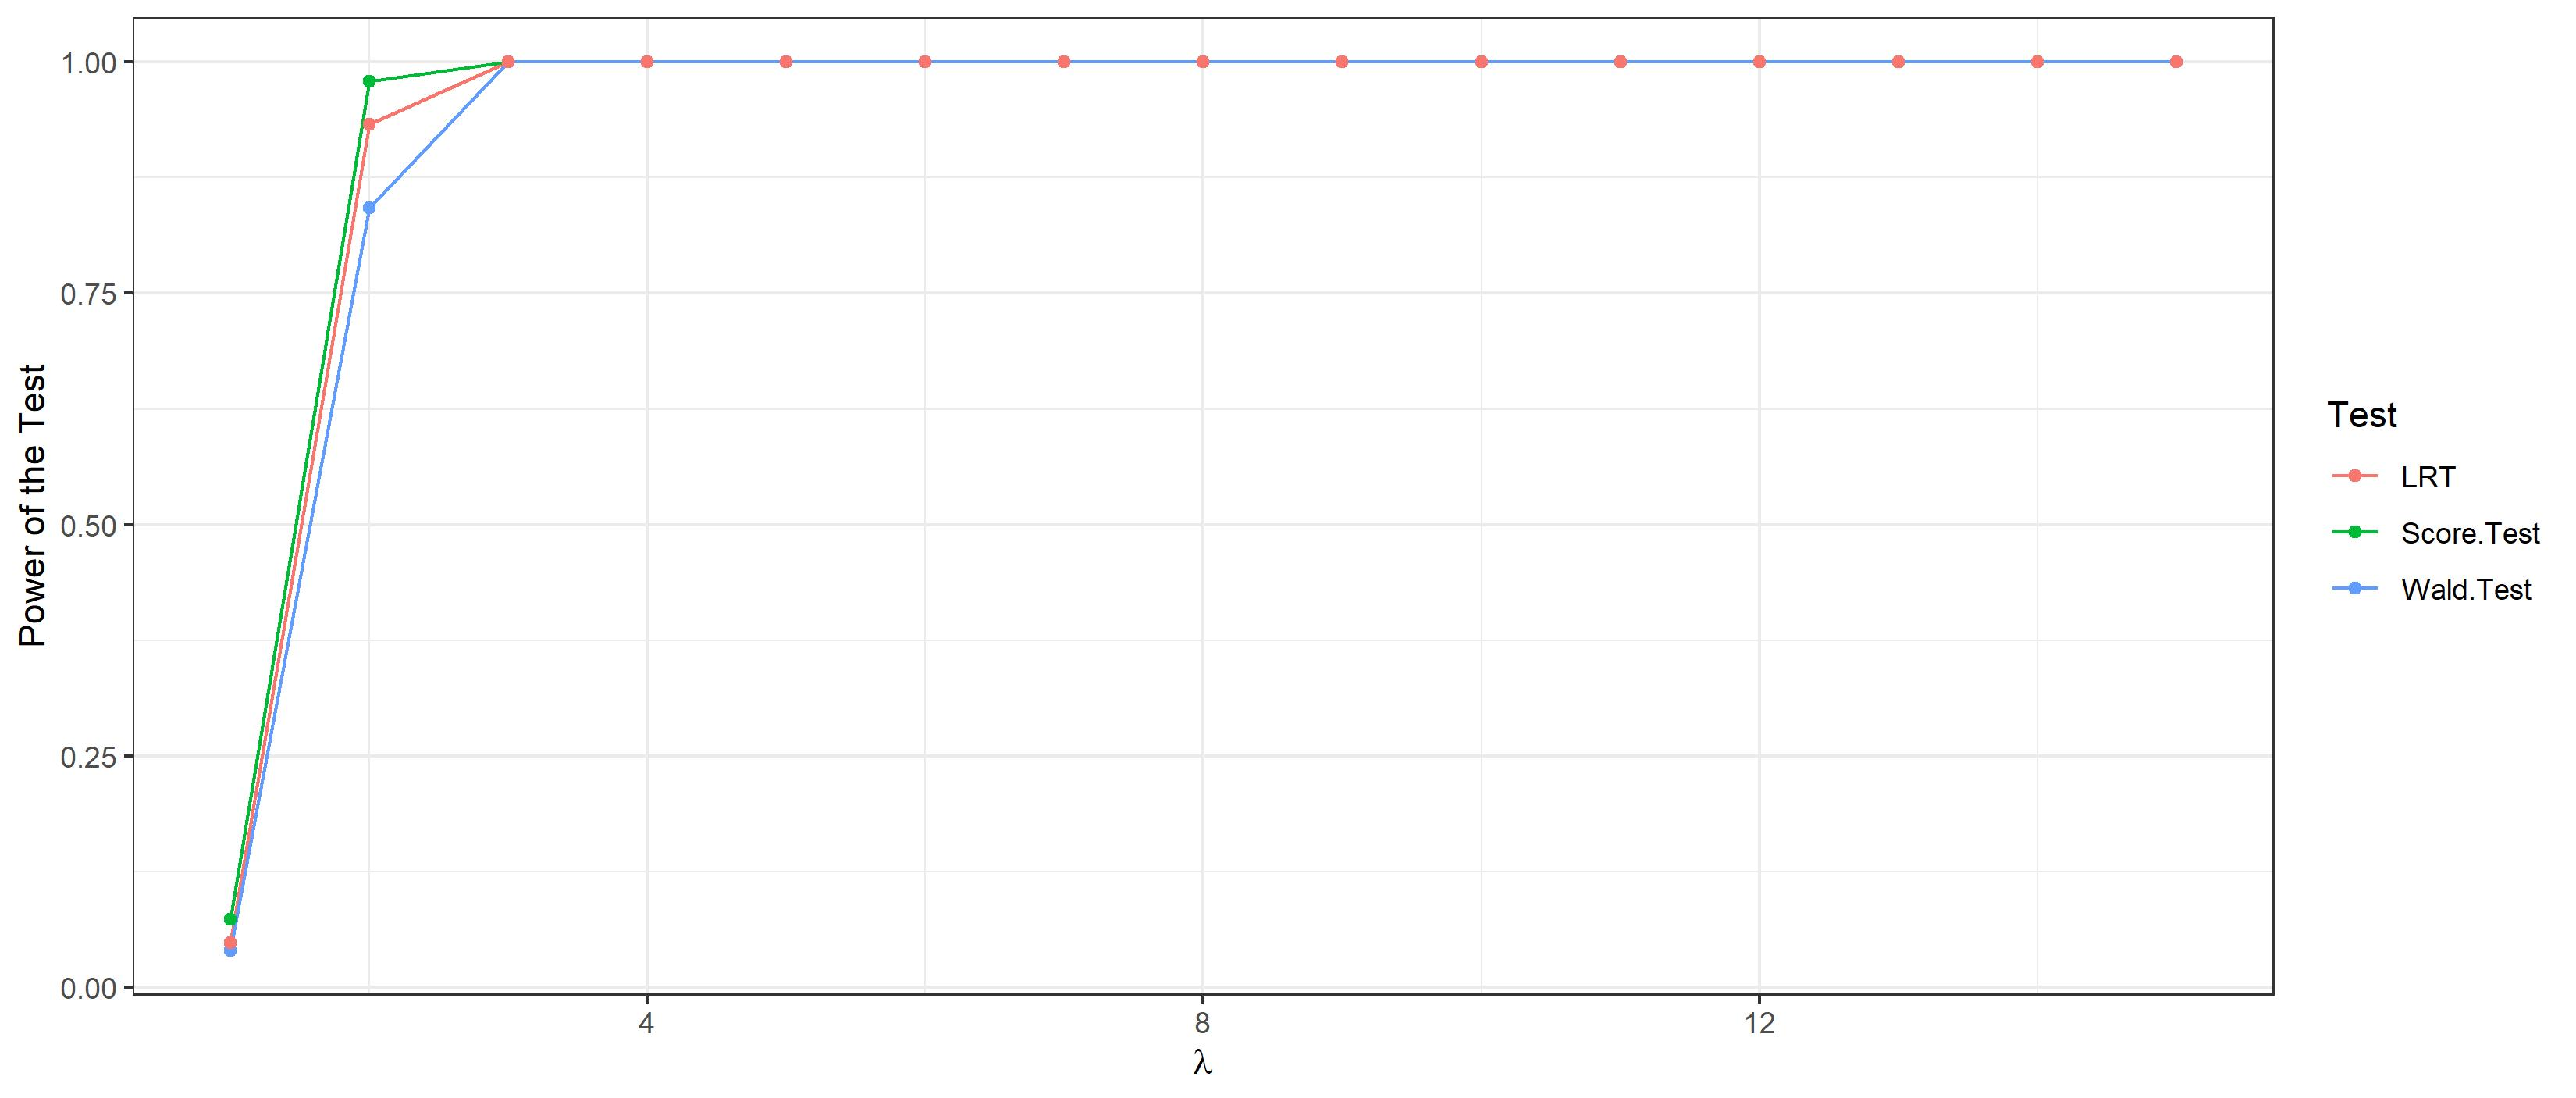
\includegraphics[width = \textwidth]{ExpTest-0.05-25.jpg}
            \caption{n = 25}
        \end{subfigure}
        \caption{Approximate power curve of the three asymptotic tests under $5\%$ censored data for different sample sizes}
        \label{fig:1}
    \end{figure}

    Similarly, Table~\ref{tbl:test-unif} and Table~\ref{tbl:test-weibull} contains the details of the simulation where the censoring distribution are Uniform and Weibull respectively.

    \begin{table}[ht]
        \centering
        \begin{tabular}{@{}cl|rrr|rrr@{}}
            \toprule
            \multirow{2}{*}{\begin{tabular}[c]{@{}c@{}}Proportion of\\ Censoring\end{tabular}} & \multicolumn{1}{c|}{\multirow{2}{*}{n}} & \multicolumn{3}{c|}{Approximate Size} & \multicolumn{3}{c}{Area under the power curve} \\
             & \multicolumn{1}{c|}{} & \multicolumn{1}{c}{Score test} & \multicolumn{1}{c}{Wald's test} & \multicolumn{1}{c|}{LRT} & \multicolumn{1}{c}{Score test} & \multicolumn{1}{c}{Wald's test} & \multicolumn{1}{c}{LRT} \\ \midrule
            \multirow{3}{*}{$5\%$} & 5 & 0.14 & 0.074 & 0.067 & 0.78 & 0.068 & 0.615 \\
             & 10 & 0.13 & 0.061 & 0.06 & 0.834 & 0.519 & 0.777 \\
             & 25 & 0.076 & 0.052 & 0.047 & 0.86 & 0.833 & 0.851 \\ 
            \midrule
            \multirow{3}{*}{$20\%$} & 5 & 0.142 & 0.078 & 0.065 & 0.777 & 0.067 & 0.609 \\
            & 10 & 0.124 & 0.065 & 0.058 & 0.832 & 0.512 & 0.774 \\
            & 25 & 0.067 & 0.052 & 0.044 & 0.859 & 0.83 & 0.851 \\ 
            \midrule
            \multirow{3}{*}{$40\%$} & 5 & 0.152 & 0.094 & 0.073 & 0.774 & 0.063 & 0.603 \\
            & 10 & 0.125 & 0.077 & 0.053 & 0.83 & 0.5 & 0.767 \\
            & 25 & 0.082 & 0.056 & 0.043 & 0.859 & 0.826 & 0.848 \\
            \bottomrule
        \end{tabular}
        \caption{Small sample performances of score test, Wald's test and LRT for uniform distribution as the censoring distribution.}
        \label{tbl:test-unif}
    \end{table}

    \begin{table}[ht]
        \centering
        \begin{tabular}{@{}cl|rrr|rrr@{}}
            \toprule
            \multirow{2}{*}{\begin{tabular}[c]{@{}c@{}}Proportion of\\ Censoring\end{tabular}} & \multicolumn{1}{c|}{\multirow{2}{*}{n}} & \multicolumn{3}{c|}{Approximate Size} & \multicolumn{3}{c}{Area under the power curve} \\
             & \multicolumn{1}{c|}{} & \multicolumn{1}{c}{Score test} & \multicolumn{1}{c}{Wald's test} & \multicolumn{1}{c|}{LRT} & \multicolumn{1}{c}{Score test} & \multicolumn{1}{c}{Wald's test} & \multicolumn{1}{c}{LRT} \\ \midrule
            \multirow{3}{*}{$5\%$} & 5 & 0.149 & 0.081 & 0.068 & 0.844 & 0.485 & 0.8 \\
             & 10 & 0.107 & 0.063 & 0.053 & 0.856 & 0.809 & 0.842 \\
             & 25 & 0.077 & 0.052 & 0.042 & 0.865 & 0.857 & 0.862 \\ 
            \midrule
            \multirow{3}{*}{$20\%$} & 5 & 0.155 & 0.083 & 0.064 & 0.845 & 0.486 & 0.801 \\
            & 10 & 0.112 & 0.06 & 0.05 & 0.856 & 0.81 & 0.843 \\
            & 25 & 0.072 & 0.048 & 0.039 & 0.865 & 0.858 & 0.862 \\ 
            \midrule
            \multirow{3}{*}{$40\%$} & 5 & 0.144 & 0.06 & 0.064 & 0.845 & 0.486 & 0.803 \\
            & 10 & 0.1 & 0.051 & 0.046 & 0.858 & 0.811 & 0.844 \\
            & 25 & 0.07 & 0.042 & 0.047 & 0.865 & 0.859 & 0.863 \\
            \bottomrule
        \end{tabular}
        \caption{Small sample performances of score test, Wald's test and LRT for Weibull distribution as the censoring distribution.}
        \label{tbl:test-weibull}
    \end{table}

    From the results shown in Table~\ref{tbl:test-exp},Table~\ref{tbl:test-unif} and Table~\ref{tbl:test-weibull}, we conclude that

    \begin{enumerate}
        \item Generally, Score test has more power than Likelihood Ratio Test (LRT) and LRT has more power than Wald's test.
        \item As the sample size $n$ increases, all of the tests perform similarly.
        \item While LRT and Wald's test have approximately $5\%$ size for small samples,  Score test usually has higher size than intended.
        \item As the proportion of censoring increases, the power of all three tests decreases when the censoring distribution is exponential or Weibull distribution. However, when the censoring distribution is uniform, the effect of the proportion of censoring is very limited.
        \item Under heavy censoring ($40\%$ censored data), Wald's test have very small power (similar to its size) for small samples. 
    \end{enumerate}

    In summary, Wald's test should not be considered if the sample size is small. Likelihood Ratio test should be preferred in such scenario.

\end{solution*}









\pagebreak
\begin{center}
    \vspace*{5cm}
    \rule{0.8\linewidth}{0.1pt}\\
    \vspace*{2cm}
    \Huge \textbf{Thank You}\\
    \vspace*{2cm}
    \rule{0.8\linewidth}{0.1pt}
    \vfill
\end{center}


\end{document}